%%
%% @filename TD2.tex
%% @date lun. 16 nov. 2020 09:47:34 CET
%% @author Guillaume Fornes <guillaume.fornes@enseirb-matmeca.fr>
%%
\documentclass[a4paper]{article}

\usepackage[utf8]{inputenc}
\usepackage[french]{babel} 

% Figures
\usepackage{graphicx}
\graphicspath{{./img/}}

% Math
\usepackage{amsmath, amssymb}
\newtheorem{defi}{Définition}

% Algortihmes
\usepackage[vlined,lined,linesnumbered,boxed,french]{algorithm2e}
\DeclareMathOperator*{\argmin}{argmin}
\DeclareMathOperator{\myfunc}{myfunc}
\DeclareMathOperator*{\sign}{sign}
\DeclareMathOperator*{\imwh}{width}
\DeclareMathOperator*{\imht}{height}

% Extra
\usepackage[left=2cm,right=2cm,top=2cm,bottom=2cm]{geometry}
\usepackage{url}
\usepackage{setspace}

\begin{document}

\section*{TD2 - Logique des prédicats}
\begin{spacing}{1.25}
\subsection*{Exercice 1}
\begin{figure}[!h]
  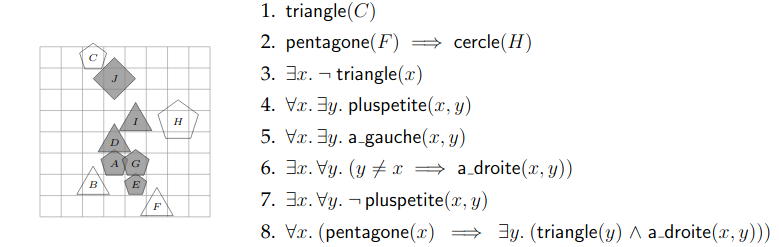
\includegraphics[scale = 0.67]{ex1_td2}
\end{figure}
\begin{enumerate}
  \item  FAUX
  \item VRAI
  \item VRAI
  \item FAUX
  \item FAUX
  \item VRAI
  \item VRAI
  \item FAUX
\end{enumerate}

\subsection*{Exercice 2}
\begin{enumerate}
  \item $\exists x.P(x) \equiv p(a)\lor p(b) \lor p(c)$\\
    $\forall x.P(x) \equiv p(a)\land p(b) \land p(c)$\\
    Si x est dans un domaine fini alors on peut éliminer les quantificateurs $\forall ,\exists$.\\
    \item $x \in \mathbb{N} , p(0)\lor p(1) \lor ...$ ,n'est pas un formule !! ($\bigvee_{x\in \mathbb{N}}p(x)$ non plus !!)\\
    On peut donc avec \emph{ $\forall \:et\: \exists $ } écrire des formules correctes.\\
\end{enumerate}
\subsection*{Exercice 3}
\begin{enumerate}
  \item $\forall x \forall y \; equipe(x,y) \iff equipe(y,x)$\\
    $\forall x \forall y \forall z \; equipe(x,y) \land equipe(y,z) \implies equipe(x,z)$\\
    $equipe(x,x) = 0$\\
  \item $\forall x . \exists y \text{ tel que } ((x\ne y)\land equipe(x,y))$ On peut se passer de $x \ne y$ car on a montrer en Q1. que l'équipe est irreflexive.\\
  \item $\forall x \forall y \; (equipe(x,y) \implies meme\_club(x,y))$\\
  \item $(\forall x \exists y (equipe(x, y) \land (femme(x) \implies \lnot femme(y)) \land (\lnot femme(x) \implies femme(y)))$\\
  \item $\forall x \forall y\; equipe(x,y) \implies (\exists z .(z \ne y \land  z \ne x \land equipe(x,z)))$ \emph{ligne peut-être/sûrement fausse}\\
    $\forall x (\exists y . equipe(x,y)) \hdots $ \emph{problème d'incohérence de l'exercice.}\\
\end{enumerate}
\subsection*{Exercice 4}
\begin{enumerate}
  \item $\exists idc \: . \: client(idc, \; nom)$\\
  \item $\exists idc \: (client(idc, \; nom) \land \exists idp \: . \: vente(idp,\; idc) \land produit(idp, \; shampooing )) $\\
  \item $\forall idp \; (produit(idp, \; description)\implies \forall idc \; \lnot vente(idp, \; idp))$\\
\end{enumerate}
\subsection*{Exercice 5}
\begin{enumerate}
  \item $(\forall x . \lnot p(x)) \lor (\exists x . p(x))$ : 2 occurences liés + formule valide $(\equiv A \lor \lnot A)$.\\
  \item $p(x) \implies (\forall x . p(x))$ occurences : 1\ier libre, 2\ieme liée. formule satisfiable non valide.\\
  \item
  \item
  \item
  \item $\forall (x . p(x) \land q(x)) \iff (\forall x . p(x)) \land (\forall x.q(x))$ 4 occurences liés, formule valide.
  \item
  \item$\forall x . (p(x)\lor q(x)) \implies (\forall x .p(x)) \lor (\forall x . q(x))$ 4 occurences liés, formule satisfiable et non valide.
  \item
  \item
  \item
\end{enumerate}
\end{spacing}
\end{document}
